%%%%%%%%%%%%%%%%%%%%%%%%%%%%%%%%%%%%%%%%%%%%%%%%%%%%%%%%%%%%%%%%%%%%%%%%
%                                                                      %
%     File: Thesis_VisualSolution.tex                                 %
%     Tex Master: Thesis.tex                                           %
%                                                                      %
%     Author: Miguel Fonseca                                           %
%     Last modified : 8 Jul 2015                                       %
%                                                                      %
%%%%%%%%%%%%%%%%%%%%%%%%%%%%%%%%%%%%%%%%%%%%%%%%%%%%%%%%%%%%%%%%%%%%%%%%

\chapter{Visible Spectrum Solution}
\label{chapter:passive}

A fundamental step in sense and avoid is the increase of UA visibility. Has shown in section \ref{section:saaprograms}, there are several systems that use the visible spectrum to detect intruders which would benefit from this increase. Adding to this, it is of utmost importance to allow pilots of manned aircraft to detect these small vehicles: small unmanned aircraft will mainly operate in non-controlled airspace, which is used by aircraft that usually do not possess equipment to help the practice of see and avoid, such as TCAS. Because of this, their only way to detect intruders is visually.\\
An easy way to improve the visual detectability of sUA is to implement a position and anti-collision lights system similar to the one used by GA with requirements proportional to the aircraft type and size. As mentioned in section \ref{subsubsection:poslights}, this system increases the probability of an aircraft being detected by another aircraft crew or another SAA system which relies on radiation from the visible spectrum. The position lights also provide some information about the intruder aircraft's route.\\
As the UA studied in this thesis are much smaller and usually do not travel as fast, they don't need to be detected as far away as GA. It is then possible to adapt the visibility requirements present in CS-23 for Normal, Utility, Aerobatic and Commuter Category Airplanes to provide a desired lower consumption, as sUAs have batteries with low capabilities, and will also allow the use of smaller, lighter and cheaper lights and materials.

\section{Differentiate unmanned from manned aircraft}
\label{section:differentiateunmanned}
Instead of just identifying a sUA as an aircraft, it would provide important information to other airspace users if the used system could identify it as an unmanned aircraft.\\
For Anti-Collision Lights, CS-23 only defines a flashing frequency interval, not a pattern. To provide a way to differentiate manned and unmanned aircraft, a specific pattern of flashing may be adopted.\\
A common way of communication with visual lights is the Morse Code. Initially developed by the American artist Samuel Morse, the Morse code was used to transmit natural language through an electrical telegraph system. The system used pulses of electric current to control the receiving electromagnet that would create indentations on a paper tape.\\
The International Telecommunication Union standard Morse code \citep{ITU2009} establishes the format of the code using dots, dashes and intervals between them. A word, such as \textit{example}, is divided in letters (\textit{e}, \textit{x}, \textit{a}, \textit{m}, \textit{p}, \textit{l} and \textit{e}), which are then coded into different combinations of dots and dashes (x = '\_ . . \_' ). The different symbols can be related to each other by their duration: the dot is the shortest one and is composed by what will be called one element. The duration of the other symbols can be seen in table \ref{tab:morsesymbols}.
\begin{table}[!htb]
\centering
\caption[Morse code symbols and their duration \citep{ITU2009}]{Morse code symbols and their duration \citep{ITU2009}}
\label{tab:morsesymbols}
\begin{tabular}{@{}llll@{}}
\toprule
Symbol & Name         & Utilization                                   & No. of Elements \\ \midrule
.      & dot          &                                               & 1               \\
\_     & dash         &                                               & 3               \\
{[}{]} & inter-symbol & space between symbols forming the same letter & 1               \\
()     & inter-letter & space between letters                         & 3               \\
\{\}   & inter-word   & space between words                           & 7               \\ \bottomrule
\end{tabular}
\end{table}

With the adoption of Morse code for radio communications, the aviation world started to use it for both communication and the identification of navigational beacons, know as Non-Directional Beacons (NDBs), which continuously transmitted unique identifiers in Morse code. The transmitted signal would be received by a manually controlled antenna that, in association with the aircraft's magnetic compass, would provide the pilot with the aircraft's bearing from the NDB \citep{Nolan2010}. The pilot could then obtain the aircraft's position by plotting the bearing of two different NDBs.\\
Although Morse Code's use for radio communication and distress signals has decreased, it is still used to allow the identification and evaluation of the state of operation of air navigation aids \citep{FederalAviationAdministration2015a}, so pilots should still be able to recognize and correctly interpret Morse Code.
\subsection{Aircraft types}
\label{subsection:aircraftypes}
Using Morse Code, an aircraft can repeatedly transmit an identification code or letter. This code should not only identify an aircraft as manned or unmanned but also its type, such as light aircraft or military jets. An example of such categorization was adapted from \citep{Angelov2012} and \citep{Eurocontrol2010}: 
\begin{itemize}
\item A - Unpowered air sports (hang gliders, etc...)
\item B - Hot air balloons
\item C - Cargo aircraft or military air transport
\item D - Dirigible airships
\item E - Emergency
\item H - Helicopters and other rotorcraft
\item K - Kites and tethered balloons
\item L - Light aircraft
\item M - Military fighters and high-performance jets
\item N - Pressurized passenger aircraft not required to carry ACAS
\item Q - Pressurized general aviation with a maximum take-off mass (MTOM) less than 5700 kg
\item R - Radio-controlled model aircraft operated by hobbyists
\item S - Powered air sports (ultra-lights, etc...)
\item T - Pressurized passenger aircraft required to carry ACAS
\item U - Unmanned aircraft
\end{itemize}
The E for Emergency was added as requested in paragraph 4.2.2.4 of \citep{Eurocontrol2010}.\\
An unmanned dirigible would then transmit the word \textit{UD}, while a manned helicopter during an emergency should transmit the word \textit{E} and an ultra-light will use the word \textit{S}.
\subsection{Generating the Morse Code}
\label{subsection:generatemorse}
In the studied case, a dash represents a flash with a duration equal to three times the duration of a dot.\\
The used Morse code must have a flashing pattern according to international requirements for anti-collision lights but it must also use a flashing velocity that enables pilots to see it and understand the code. To enable this, the flashing velocity used will be the same as the transmission speed of Non-Directional Beacons. As previously discussed, NDBs transmit a call-sign in Morse code which allows pilots to identify the NDB by comparing the signal to the information displayed in navigation charts. ICAO defines the communication velocity of NDBs as 7 words per minute \citep{InternationalCivilAviationOrganization2006}.\\

To identify the correct period for each element, two strategies can be adopted. The first uses the ICAO defined communication velocity for each category, adapting the flashing velocity to achieve the required 7 words per minute. The second uses a standard word to correct flashing times.\\
The signal transmitted by a category \textit{H} manned aircraft and an unmanned aircraft which also belongs to the \textit{H} category would then be respectively composed by the following two words:
\begin{itemize}
  \item[] H = . . . . = 1+[1]+1+[1]+1+[1]+1+\{7\} = 14 elements
  \item[] UH = . . \_ \space\space\space . . . . = 1+[1]+1+[1]+3+(3)+1+[1]+1+[1]+1+[1]+1+\{7\} = 24 elements
\end{itemize}
The number of elements per word for every category can be seen in table \ref{tab:morsefrequency1}, for either manned (x) and unmanned (\textit{U}x) aircraft.\\
For the first method, multiplying the number of elements per word with the defined communication velocity of 7 words per minute, we obtain the number of elements per minute for each category. Next, dividing 60 by the number of elements per minute, we obtain the correct element's period for each transmitted message, as shown in table \ref{tab:morsefrequency1}.
\begin{table}[!htb]
\centering
\caption[Morse code symbols with the respective number of elements and the element's period]{Morse code symbols with the respective number of elements and the element's period}
\label{tab:morsefrequency1}
\begin{tabular}{@{}lllllll@{}}
\toprule
\multicolumn{1}{c}{\multirow{3}{*}{Category and Morse Code}} & \multicolumn{4}{c}{Number of elements}                        & \multicolumn{2}{c}{\multirow{2}{*}{Element's Period (s)}} \\ \cmidrule(lr){2-5}
                                         & \multicolumn{2}{c}{Per Word} & \multicolumn{2}{c}{Per Minute \#1} & \multicolumn{2}{c}{}                                      \\ \cmidrule(l){6-7} 
                                         & Manned       & Unmanned      & Manned        & Unmanned       & Manned                     & Unmanned                     \\ \cmidrule(r){1-1}
A . \_                                   & 12           & 22            & 84            & 154            & 0,714                      & 0,390                        \\
B \_ . . .                               & 16           & 26            & 112           & 182            & 0,536                      & 0,330                        \\
C \_ . \_ .                              & 18           & 28            & 126           & 196            & 0,476                      & 0,306                        \\
D \_ . .                                 & 14           & 24            & 98            & 168            & 0,612                      & 0,357                        \\
E .                                      & 8            & 18            & 56            & 126            & 1,071                      & 0,476                        \\
H . . . .                                & 14           & 24            & 98            & 168            & 0,612                      & 0,357                        \\
K \_ . \_                                & 16           & 26            & 112           & 182            & 0,536                      & 0,330                        \\
L . \_ . .                               & 16           & 26            & 112           & 182            & 0,536                      & 0,330                        \\
M \_ \_                                  & 14           & 24            & 98            & 168            & 0,612                      & 0,357                        \\
N \_ .                                   & 12           & 22            & 84            & 154            & 0,714                      & 0,390                        \\
Q \_ \_ . \_                             & 20           & 30            & 140           & 210            & 0,429                      & 0,286                        \\
R . \_ .                                 & 14           & 24            & 98            & 168            & 0,612                      & 0,357                        \\
S . . .                                  & 12           & 22            & 84            & 154            & 0,714                      & 0,390                        \\
T \_                                     & 10           & 20            & 70            & 140            & 0,857                      & 0,429                        \\
U . . \_                                 & 14           & -             & -            & -              & -                          & -                            \\ \bottomrule
\end{tabular}
\end{table}

The second approach defines "PARIS" as the standard word to calculate the correct flashing times \citep{Morsh1948}:
\begin{itemize}
  \item[] P = . \_ \_ . = 1+[1]+3+[1]+3+[1]+1+(3) = 14 elements             
  \item[] A = . \_ = 1+[1]+3+(3) = 8 elements              
  \item[] R = . \_ . = 1+[1]+3+[1]+1+(3) = 10 elements			  
  \item[] I = . . = 1+[1]+1+(3) = 6 elements			  
  \item[] S = . . . = 1+[1]+1+[1]+1+\{7\} = 12 elements	  
  \item[] Total = 50 elements		 
\end{itemize}
With 50 elements per word and 7 words per minute, as used by NDBs, we obtain 350 elements per minute, or a period of 0.171 seconds per element.\\
Dividing the PARIS number of elements per minute (350) by the number of elements per word of each category, we get the number of words per minute. Then, to obtain the number of flashes per minute using the PARIS standard (method \#2), we multiply the number of elements per minute by the number of flashes per word. The results are shown in table \ref{tab:morsefrequency2}.\\
The number of flashes per minute \#1 is calculated according to the first approach, where each word should be transmitted exactly 7 times per minute.
\begin{table}[!htb]
\centering
\caption[Morse code symbols with number of flashes per word and per minute for each approach]{Morse code symbols with number of flashes per word and per minute for each approach}
\label{tab:morsefrequency2}
\begin{tabular}{@{}lllllll@{}}
\toprule
\multicolumn{1}{c}{\multirow{3}{*}{Category and Morse Code}} & \multicolumn{6}{c}{Number of flashes}                                                                                                                                              \\ \cmidrule(l){2-7} 
\multicolumn{1}{c}{}                                         & \multicolumn{2}{c}{Per word}                              & \multicolumn{2}{c}{Per minute \#1}                        & \multicolumn{2}{c}{Per minute \#2}                        \\
\multicolumn{1}{c}{}                                         & \multicolumn{1}{c}{Manned} & \multicolumn{1}{c}{Unmanned} & \multicolumn{1}{c}{Manned} & \multicolumn{1}{c}{Unmanned} & \multicolumn{1}{c}{Manned} & \multicolumn{1}{c}{Unmanned} \\ \cmidrule(r){1-1}
A . \_                                                       & 2                          & 5                            & 14                         & 35                           & 58,33                      & 79,55                        \\
B \_ . . .                                                   & 4                          & 7                            & 28                         & 49                           & 87,50                      & 94,23                        \\
C \_ . \_ .                                                  & 4                          & 7                            & 28                         & 49                           & 77,78                      & 87,50                        \\
D \_ . .                                                     & 3                          & 6                            & 21                         & 42                           & 75,00                      & 87,50                        \\
E .                                                          & 1                          & 4                            & 7                          & 28                           & 43,75                      & 77,78                        \\
H . . . .                                                    & 4                          & 7                            & 28                         & 49                           & 100,00                     & \textbf{102,08                      } \\
K \_ . \_                                                    & 3                          & 6                            & 21                         & 42                           & 65,63                      & 80,77                        \\
L . \_ . .                                                   & 4                          & 7                            & 28                         & 49                           & 87,50                      & 94,23                        \\
M \_ \_                                                      & 2                          & 5                            & 14                         & 35                           & 50,00                      & 72,92                        \\
N \_ .                                                       & 2                          & 5                            & 14                         & 35                           & 58,33                      & 79,55                        \\
Q \_ \_ . \_                                                 & 4                          & 7                            & 28                         & 49                           & 70,00                      & 81,67                        \\
R . \_ .                                                     & 3                          & 6                            & 21                         & 42                           & 75,00                      & 87,50                        \\
S . . .                                                      & 3                          & 6                            & 21                         & 42                           & 87,50                      & 95,45                        \\
T \_                                                         & 1                          & 4                            & 7                          & 28                           & \textbf{35,00}                      & 70,00                        \\
U . . \_                                                     & 3                          & -                              & -                          & -                            & -                      & -                              \\ \bottomrule
\end{tabular}
\end{table}

As can be seen in table \ref{tab:morsefrequency1}, the obtained values for the element's period, with the first approach, range from 0.29 to 1.07 seconds. This is a high variation in the flashing frequency, which can generate incorrect receptions. Adding to this, the number of flashes per minute \#1 for most messages is not within the required effective flashing frequency for anti-collision light system stated in CS-23 \citep{Easa2012}, as can be seen in table \ref{tab:morsefrequency2}, which is between 40 and 100.\\
On the other hand, as table \ref{tab:morsefrequency2} shows, there are two instances where the number of flashes per minute \#2 is outside the limit given by the CS-23 \citep{Easa2012} (between 40 and 100) when using the PARIS standard: the manned aircraft of category T, with too few flashes, and the unmanned aircraft of category H, which has more than 100 flashes. It is possible to correct this, without interfering too much with the reception of the signal, by changing the flashing frequency just enough to have the required number of flashes per minute. In the manned T category aircraft, raising the number of flashes per minute to 40, and reducing to 100 for the unmanned H category aircraft. The resulting element's periods are shown in table \ref{tab:morsefrequency3}.
\begin{table}[!htb]
\centering
\caption[Correction of the number of flashes per minute for aircraft of type H and T]{Correction of the number of flashes per minute for aircraft of type H and T}
\label{tab:morsefrequency3}
\begin{tabular}{@{}lllllll@{}}
\toprule
\multirow{3}{*}{Category and Morse Code} & \multicolumn{2}{c}{\multirow{2}{*}{\begin{tabular}[c]{@{}c@{}}Number of Flashes\\ per Minute \#2\end{tabular}}} & \multicolumn{2}{c}{\multirow{2}{*}{\begin{tabular}[c]{@{}c@{}}Number of Elements\\ per Minute \#2\end{tabular}}} & \multicolumn{2}{c}{\multirow{2}{*}{Element's Period (s)}} \\
                                         & \multicolumn{2}{c}{}                                                                                             & \multicolumn{2}{c}{}                                                                                              & \multicolumn{2}{c}{}                                      \\ \cmidrule(l){2-7} 
                                         & Manned                                                 & Unmanned                                                & Manned                                                 & Unmanned                                                 & Manned                     & Unmanned                     \\ \cmidrule(r){1-1}
H . . . .                                & 100                                                    & 100                                                     & 350                                                    & 343                                                      & 0,171                      & 0,175                        \\
T \_                                     & 40                                                     & 70                                                      & 400                                                    & 350                                                      & 0,150                      & 0,171                        \\ \bottomrule
\end{tabular}
\end{table}

\subsection{Lights configuration and range}
\label{subsection:lightsrange}

Because unmanned aircraft may display several different configurations, it is difficult to define a position and anti-collision lights system for each and every type. For example, small multicopters, are able to quickly change their flight direction. Even so, they usually have a standard front side, as helicopters, or the pilot would quickly loose control of the aircraft. Having this in consideration, the position lights system for unmanned aircraft should have a configuration as is defined by EASA \citep{Easa2012} and mentioned in section \ref{subsubsection:poslights}, where the standard front side is used as reference to the lights. In figure \ref{fig:esquemalights2} two types of aircraft are shown with similar position and anti-collision lights systems.

\begin{figure}[!htb]
  \centering
  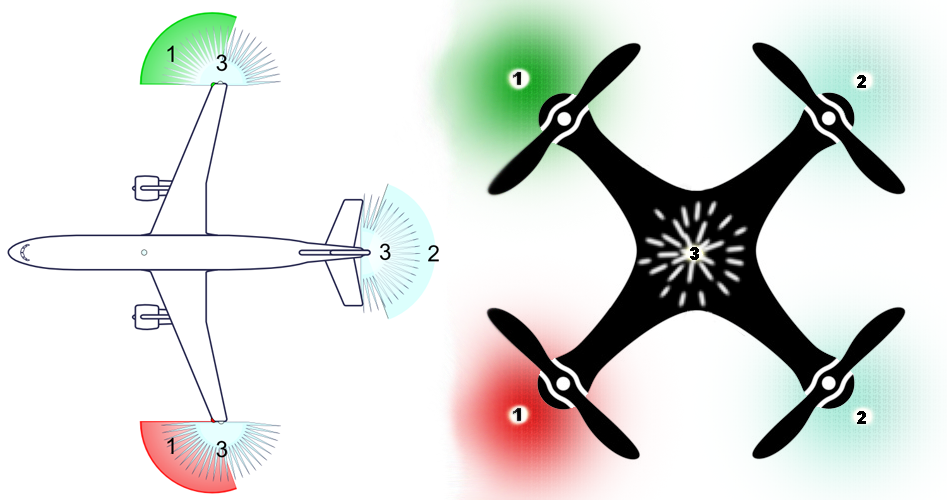
\includegraphics[width=0.90\textwidth]{Figures/esquemalights2.png}
  \caption[Configuration of Position and Anti-Collision for Two Different Aircraft]{Configuration of Position and Anti-Collision for Two Different Aircraft (1-left and right position lights; 2-rear position lights; 3-anti-collision lights}
  \label{fig:esquemalights2}
\end{figure}

The lights range is restricted by the battery power, which usually grants electric power to all the systems inside a sUA. If the selected LEDs consume too much current, the aircraft's maximum time of operation might decrease several minutes. Adding to this, as this thesis is focused in small unmanned aircraft, it is important that the required equipment does not present a high cost to the owner of the equipment, as it would not be cost effective to use a position lights system that costs as much or even more than the rest of the equipment. It may not also present large dimensions and/or weight, so that it does not have a big negative impact in the sUA's overall operation. Finally, the equipment must be accessible, so that any owner can easily buy it: the studied materials should be acquired from stores that are open to the general public and not directly from manufacturers.\\
With this restrictions, it is expected that the required intensities and/or field coverage \citep{Easa2012} will not be met. Because of this, a relation between the characteristics of the aircraft and the required intensities must be developed. \\

As stated in the European Union's Commission Regulation No 859/2008 \citep{EuropeanCommission2008}, the minimum flight visibility limit for aircraft operating in Classes A, B, C, D and E bellow 3050 m and Class G is 5 km. Using this distance as the required range for the proposed position and anti-collision lights system and taking in consideration that sUA travel at a fraction of a normal, utility, aerobatic or commuter aircraft's velocities, provides enough range for manned and unmanned aircraft to see the aircraft and avoid collision.\\
Using equation \ref{eq:intensity} \citep{UnitedStatesCoastGuard2011}, we can calculate the required intensity to achieve the selected range of visibility.\\
\begin{equation}\label{eq:intensity}
I = 3.43 \times 10^{6} \times T \times D^{2} \times K^{-D}
\end{equation}
With:
\begin{itemize}
\item I - luminous intensity in candelas
\item T - threshold factor = $2\times 10^{-7}$ lux
\item D - range of visibility in nautical miles
\item K - atmospheric transmissivity = $0.9$
\end{itemize}
Knowing that 5 km is approximately 2,7 nm, the required intensity is 6.65 cd.\\

Although it may prove difficult to find LEDs with the right field coverage and luminous intensity for the different types of lights (left, right, etc...), it is indispensable that the entire 360\degree are covered and that the limits for each type of light are respected. A possible solution is to use LEDs with a smaller field coverage and to overlap the LEDs of the same type.\\

\section{Material}
\label{section:pmaterial}

To enable the requirements cited in the previous section, the material will be chosen from local electronics stores with websites.\\

\subsection{Selecting LEDs}
The LEDs selected for position lights should have low viewing angles, to enable control of the field of coverage according to CS-23 \citep{Easa2012} and have higher intensities while consuming less power.\\
Due to the bigger field of coverage required for the anti-collision light, the selected LED must have a high viewing angle, while still transmitting with high intensities.\\
The number of LEDs for each position light must be enough to achieve the required field coverage \citep{Easa2012}.\\

The LEDs selected for the left and right position lights are the 5mm Super Bright Red/Green LEDs with part number WW05A3SRP4-N2 and WW05A3SGQ4-N2, respectively, from Wah Wang Holdings. Both have a viewing angle of 25\degree and a forward current of 20 mA. The red LED has a dominant wavelength between 620 and 630 nm, a typical luminous intensity of 8200 mcd and a forward voltage of 2.1 V. The green LED has a dominant wavelength between 515 and 525 nm, a typical luminous intensity equal to 18000 mcd and a forward voltage of 3.1 V. More information can be seen in the respective data sheet \citep{WahWangHoldingsCo.LTD} \citep{WahWangHoldingsCo.LTDb}.\\
The LED selected for the rear position light is the 5mm Super Bright White LED with part number WW05C3SWQ4-N1 from Wah Wang Holdings. With a viewing angle of 20\degree and a forward current of 20 mA, it typically radiates with a luminous intensity equal to 18000 mcd and a forward voltage of 3.1V. More information can be seen in the data sheet \citep{WahWangHoldingsCo.LTDa}.\\
The LED selected for the anti-collision light is the Super Flux Pure White LED with part number OSWA4EZ2C1P-HCRI from OptoSupply. The viewing angle is equal to 120\degree and, with a forward current of 90 mA, it typically radiates with a   luminous intensity of 12000 mcd and a forward voltage equal to 3.1 V. More information can be seen in the data sheet \citep{OptoSupply}.\\
Each LED costs around \euro{0.2}.\\

As the position lights should stay turned on since the start of the operation until the end, there is no need to connect them to the Arduino\texttrademark board. Rather, they should be independent of the designed prototype, connecting directly to the source.\\
The flashing rate of the anti-collision light will be controlled by an Arduino\texttrademark board.\\

\subsection{Selecting Arduino\texttrademark Board}
\label{subsection:arduinoAHP}
Following the Analytic Hierarchy Process (AHP) methodology, one must define several criteria and sub-criteria for the decision making process, based on the main requirements for the Arduino\texttrademark board. Each criteria was then given a relative weight regarding its relevance. All the criteria, including their relative weights, are represented in figure \ref{fig:arduinoahpperc}.\\
\begin{figure}[!htb]
  \centering
  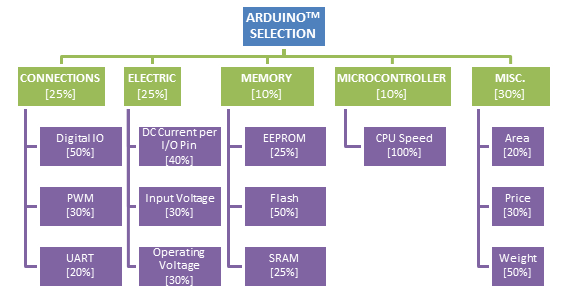
\includegraphics[width=0.90\textwidth]{Figures/arduinoahpperc.png}
  \caption[AHP study hierarchy and criteria relative weights]{AHP study hierarchy and criteria relative weights}
  \label{fig:arduinoahpperc}
\end{figure}
The five main criteria in the design selection process are Connections, Electric, Memory, Microcontroller and Miscellaneous. The Connections criteria accounts for the number of connections of different types (Digital In/Out and Pulse Width Modulation) and the number of Universal Asynchronous Receiver/Transmitter (UART) that enable serial communication. The Electric criteria refers to electric characteristics, such as the DC current available per In/Out pin, the recommended input voltage and the operating voltage. Memory contains three sub-criteria that evaluate the available types of memories (EEPROM, Flash and SRAM). The Microcontroller criterion evaluates the CPU speed. Finally the Miscellaneous criteria accounts for dimensional characteristics of the Arduino\texttrademark board, such as area and weight, as well as its price.\\
The most important sub-criteria is the weight, with a 15\% absolute weight, followed with the number of digital In/Out pins, with 12,5\%, the CPU speed and DC current per In/Out pin, both with 10\%, and finally the price with an absolute weight of 9\%.\\
To enable ranking each Arduino\texttrademark board, each criterion was given an individual scale, ranging from 1 (worst performance) to 3 (best performance), as show in table \ref{tab:ranking} for the 'Connections' and 'Electric' criteria, except for the Operating Voltage (which can only be 3.3 (1 point) or 5 V (3 points) and the recommended Input Voltage which can either be below (1 point) or above (3 points) 11 V.

\begin{table}[!htb]
  \centering
  \caption[AHP sub-criteria ranking for 'Connections' and 'Electric' criteria]{AHP sub-criteria ranking for 'Connections' and 'Electric' criteria}
  \includegraphics[width=0.85\textwidth]{Figures/table1.png}
  \label{tab:ranking}
\end{table}

Each Arduino\texttrademark board was graded on every individual criterion. The final results for the top three boards are shown in table \ref{tab:ahpresults}.

\begin{table}[!htb]
  \centering
  \caption[AHP results for top three boards]{AHP results for top three boards}
  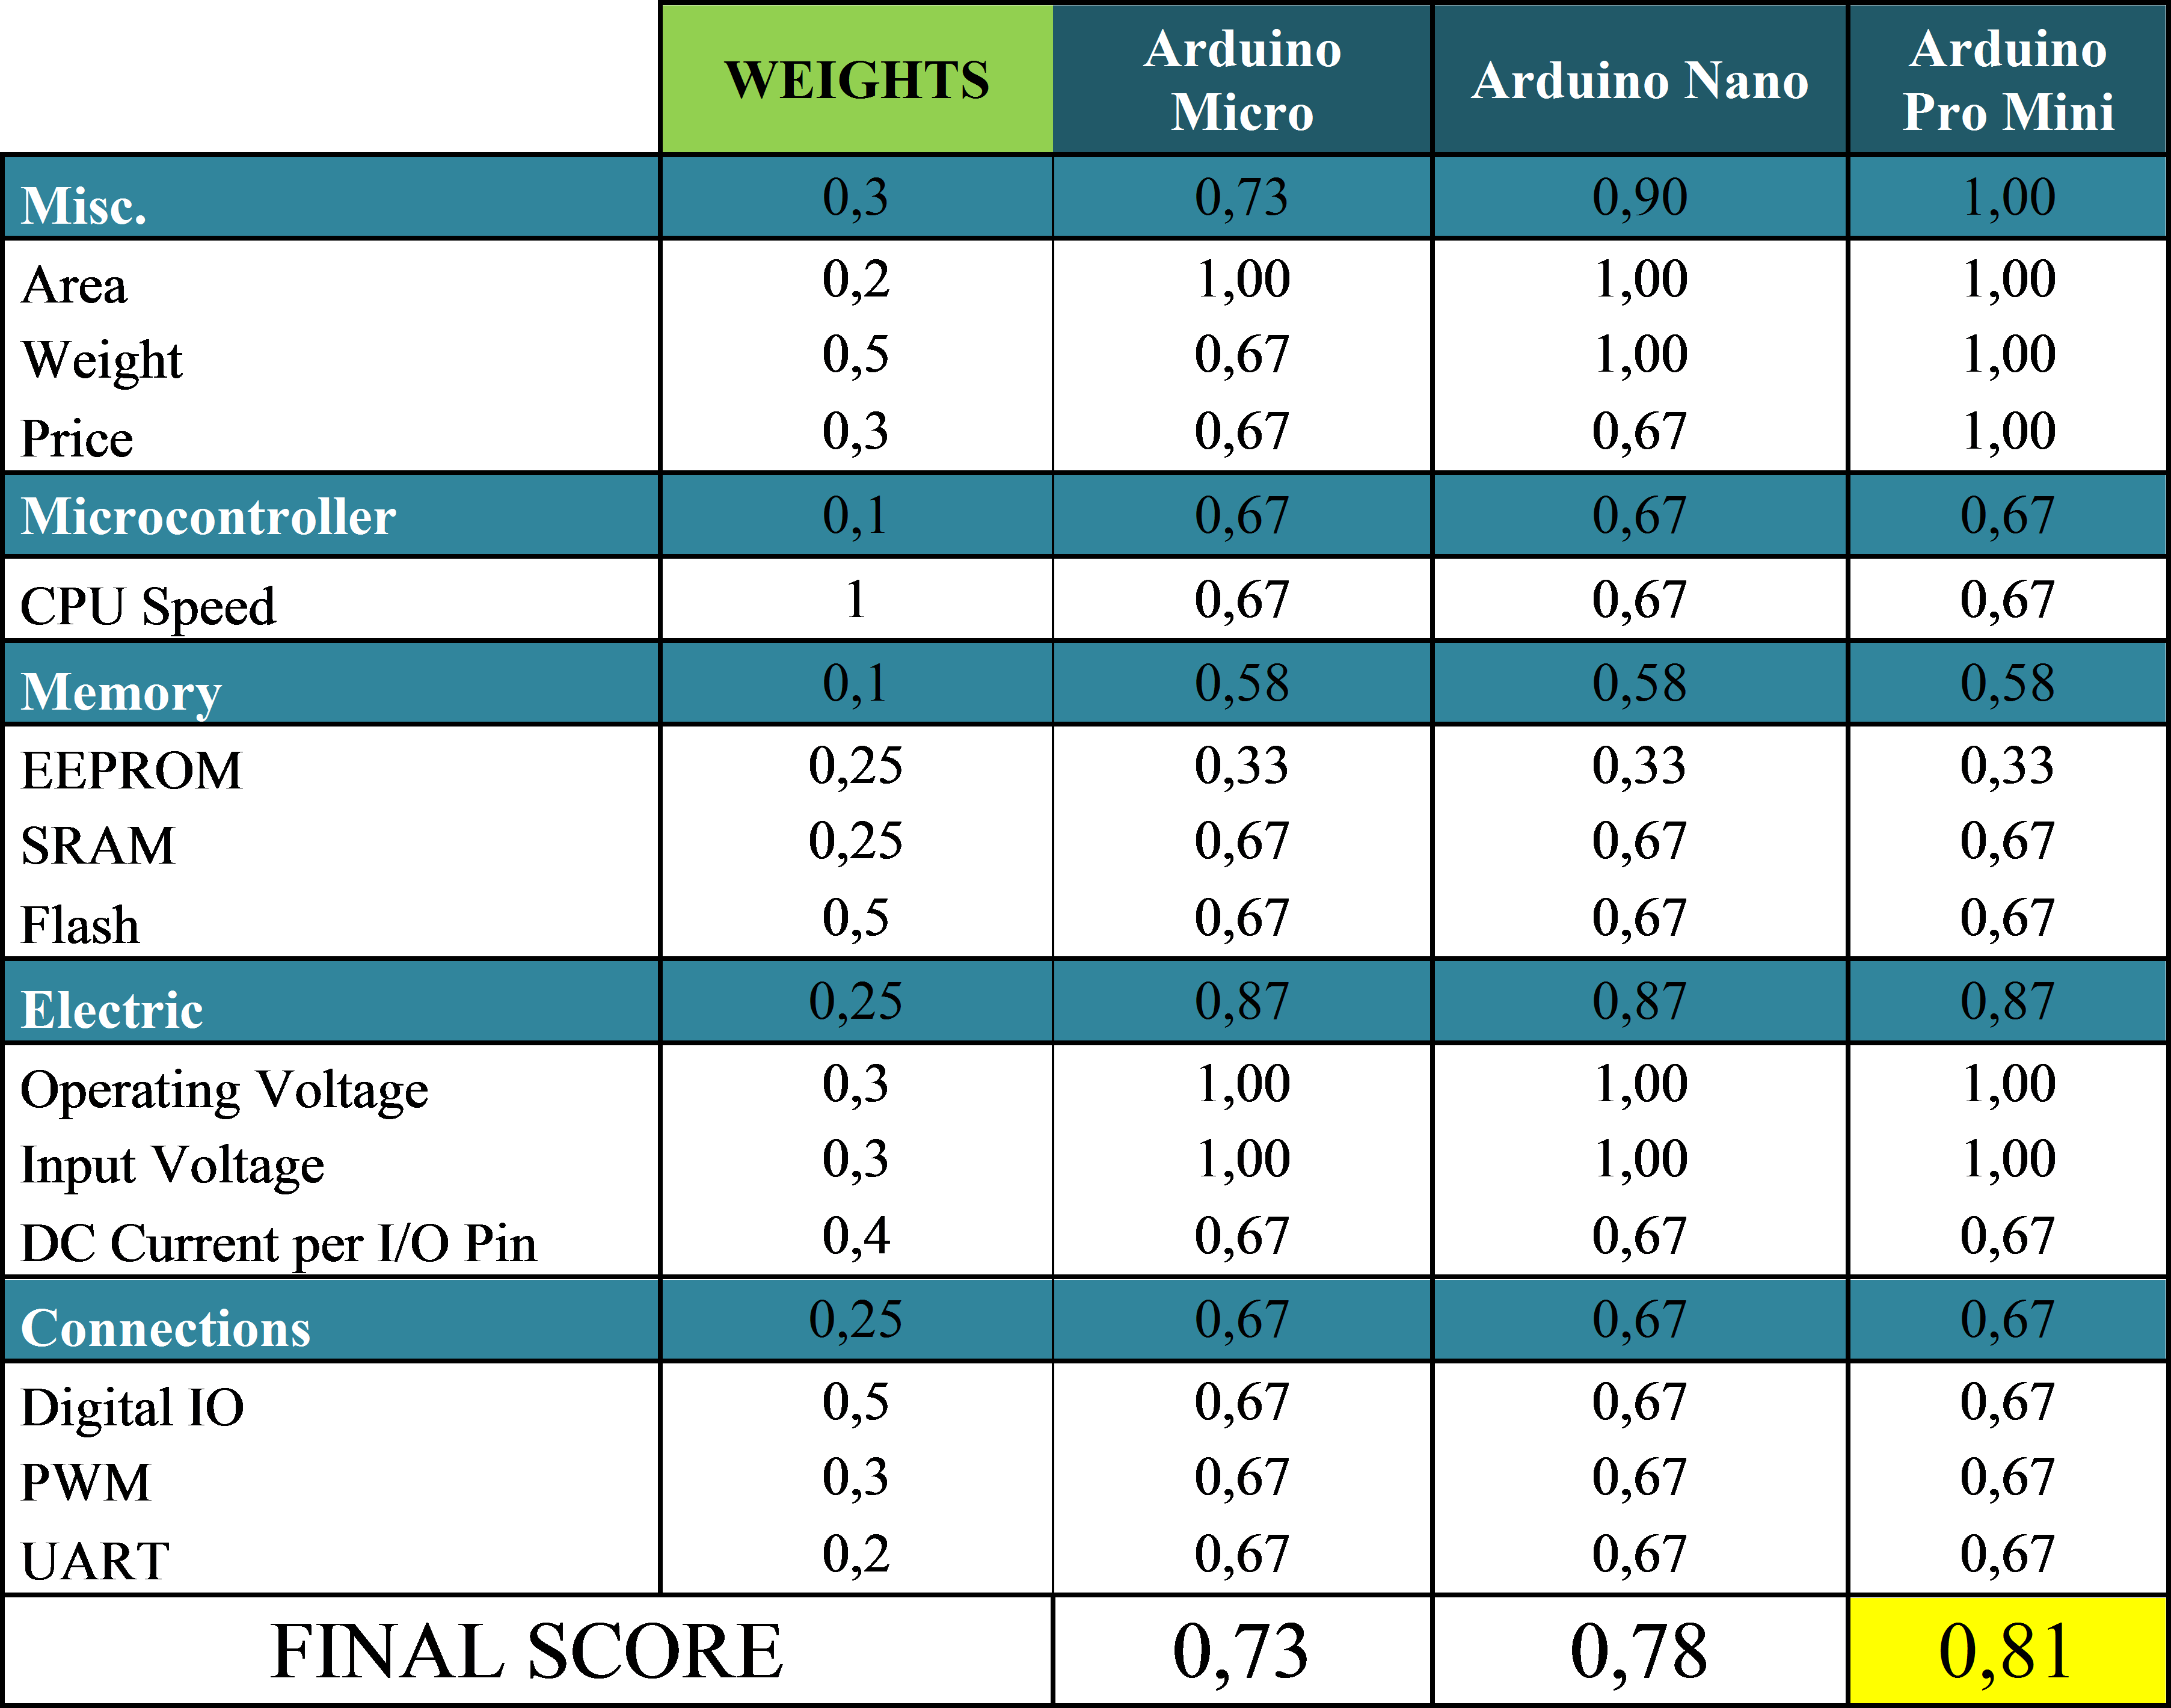
\includegraphics[width=0.75\textwidth]{Figures/ahpresults.png}
  \label{tab:ahpresults}
\end{table}

After analyzing table \ref{tab:ahpresults}, the Arduino\texttrademark board that comes on top is the Arduino\texttrademark Pro Mini which costs \euro{9.80}.\\

Because almost all Arduino\texttrademark boards, including the selected one, have a limit of 40 mA of DC current per output and the LED used for anti-collision light requires 90 mA, not enough current will be given to the LED with a direct connection between an Arduino\texttrademark board and the LED. To provide enough current, while still being able to control the flashing pattern, MOSFETs are needed to switch the LEDs. As the number of LEDs will depend on the aircraft configuration, a MOSFET with a high maximum drain current should be used.\\
The selected MOSFET is the STP55NF06, which has a drain-source-voltage of 60 V and a continuous drain current of up to 50 A. Another important characteristics are the dynamic characteristics, such as the different times. The STP55NF06 has a turn-on delay time of 20 ns, a rise time of 50 ns, a turn-off delay time of 36 ns and a fall time of 15 ns. As the signals that will be used for the anti-collision lights will have duration around several milliseconds, this MOSFET has fast enough dynamic characteristics. This MOSFET has a cost of \euro{1.17}\\
As the maximum drain current is 50 A, and each anti-collision LED is designed for 90 mA, the selected MOSFET can easily control more than 10 LEDs, which is expected to be enough for most aircraft types.\\

\subsection{Selecting resistors}
\label{subsection:resistors}
In order to obtain the desired field coverage, the number of LEDs required of each type can be seen in table \ref{tab:voltagecurrent}. To achieve the desired DC current, different configurations were adopted for each type of LED, as can be seen in figures~\ref{fig:diagrams:1}--\subref{fig:diagrams:4}: the Left Position Light will have all five LEDs in series (figure~\ref{fig:diagrams:1}), the Right Position Light will have the LEDs in one series of two and one series of three (figure~\ref{fig:diagrams:2}), the Rear Position Light will have two series of three LEDs and two series of one LED (figure~\ref{fig:diagrams:3}), and finally the Anti-Collision Light will have all three LEDs connected in series (figure~\ref{fig:diagrams:4}).\\

\begin{figure}[ht]
  \centering
  \subfigure[][]{
    \label{fig:diagrams:1} 
    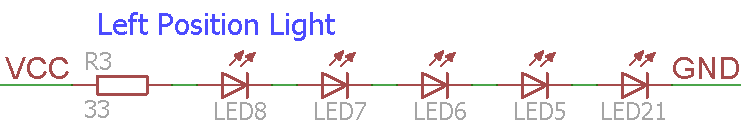
\includegraphics[]{Figures/EsquemasLights/leftpositionlight.png}
  }
  \hspace{8pt}
  \subfigure[][]{
    \label{fig:diagrams:2} 
    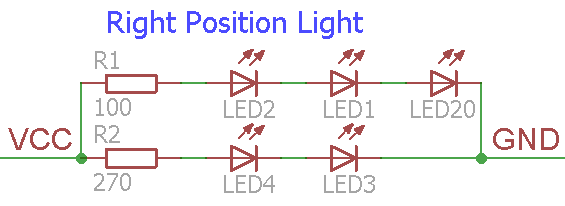
\includegraphics[]{Figures/EsquemasLights/rightpositionlight.png} 
  }\\
  \subfigure[][]{
    \label{fig:diagrams:3} 
    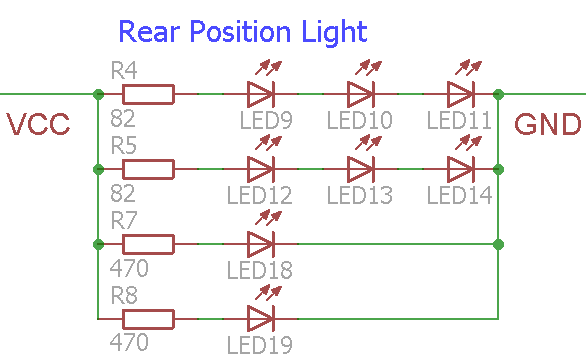
\includegraphics[]{Figures/EsquemasLights/rearpositionlight.png}
  }
  \hspace{8pt}
  \subfigure[][]{
    \label{fig:diagrams:4} 
    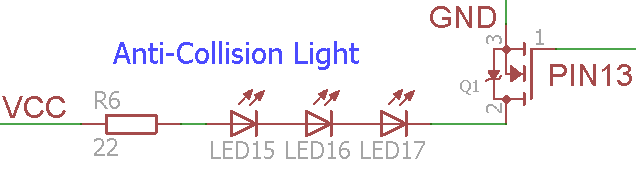
\includegraphics[]{Figures/EsquemasLights/anticollisionlight.png} 
  }
  \caption[Schematic Diagram of each Light]{Schematic Diagram of each Light:
			\subref{fig:diagrams:1} describes the Left Position Light;
			\subref{fig:diagrams:2} describes the Right Position Light;
			\subref{fig:diagrams:3} describes the Rear Position Light; and,
			\subref{fig:diagrams:4} describes the Anti-Collision Light.}%
  \label{fig:diagrams}%
\end{figure}

The required resistances are then calculated in order to obtain the correct current in each LED, using easily available resistance values. As the aircraft used for testing uses a 3S battery (11.1V), to correctly dimension the connections, we have the forward voltage and continuous forward current for each LED and the number of LEDs of each type in table \ref{tab:voltagecurrent}.\\
\begin{table}[!htb]
\centering
\caption[Forward Voltage, Continuous Forward Current and Number of LEDs for each Position and Anti-Collision Light \citep{OptoSupply}\citep{WahWangHoldingsCo.LTD}\citep{WahWangHoldingsCo.LTDa}\citep{WahWangHoldingsCo.LTDb}]{Forward Voltage, Continuous Forward Current and Number of LEDs for each Position and Anti-Collision Light \citep{OptoSupply}\citep{WahWangHoldingsCo.LTD}\citep{WahWangHoldingsCo.LTDa}\citep{WahWangHoldingsCo.LTDb}}
\label{tab:voltagecurrent}
\begin{tabular}{@{}llll@{}}
\toprule
LED                    & Forward Voltage (V) & Continuous Forward Current (mA) & Number of LEDs \\ \midrule
Green                  & 3.1                 & 20		&	5                       \\
Red                    & 2.1                 & 20       &	5                       \\
White (Rear)           & 3.1                 & 20       &	8                       \\
White (Anti-Collision) & 3.1                 & 90       &	3                       \\ \bottomrule
\end{tabular}
\end{table}
The voltage drop across each resistor can then be calculated according to equation \eqref{eq:voltagedrop}, where each LED's forward voltage depends on the number of LEDs.
\begin{equation}\label{eq:voltagedrop}
V_{D}=V_{S}-V_{F}
\end{equation}
With:
\begin{itemize}
\item $V_{D}$ - Resistor's voltage drop
\item $V_{S}$ - source's voltage
\item $V_{F}$ - total LED's forward voltage 
\end{itemize}
According to figures~\ref{fig:diagrams:1}--\subref{fig:diagrams:4}, the total LED's forward voltage for each type is equal to:
\begin{itemize}
\item Green (series of 3)- $V_{F} = 9.3 V$
\item Green (series of 2)- $V_{F} = 6.2 V$
\item Red - $V_{F} = 10.5 V$
\item White (Rear series of 3) - $V_{F} = 9.3 V$
\item White (Rear series of 1) - $V_{F} = 3.1 V$
\item White (Anti-Collision) - $V_{F} = 9.3 V$
\end{itemize}
The obtained values for each resistor's voltage drop are shown in table \ref{tab:voltageresistance}. It is then possible to calculate the required resistance with Ohm's law, shown in equation \eqref{eq:ohm}.
\begin{equation}\label{eq:ohm}
R=\dfrac{V}{I}
\end{equation}
The results are shown in table \ref{tab:voltageresistance}.
\begin{table}[!htb]
\centering
\caption[Voltage Drop and Resistance Required for each Position Light LED's Resistor]{Voltage Drop and Resistance Required for each Position Light LED's Resistor}
\label{tab:voltageresistance}
\begin{tabular}{@{}lll@{}}
\toprule
LED                    		& Resistor's voltage drop (V) 	& Resistance ($\Omega$) \\ \midrule
Green (series of 3)    		& 1.8							& 90                   \\
Green (series of 2)    		& 4.9							& 245                   \\
Red                    		& 0.6							& 30                   \\
White (Rear series of 3)    & 1.8							& 90                    \\
White (Rear series of 1)    & 8.0							& 400                   \\
White (Anti-Collision) 		& 1.8							& 20                    \\ \bottomrule
\end{tabular}
\end{table}

The obtained values for the resistance were then changed for the nearest higher rated resistor, in order to use more available material while still protecting the LEDs:
\begin{itemize}
\item Green (series of 3)- R = 100$\Omega$
\item Green (series of 2)- R = 270$\Omega$
\item Red - R = 33$\Omega$
\item White (Rear series of 3) - R = 100$\Omega$
\item White (Rear series of 1) - R = 470$\Omega$
\item White (Anti-Collision) - R = 22$\Omega$
\end{itemize}
Each resistor as an approximate cost of \euro{0.1}.\\

\section{Material Testing}
\label{section:pmaterialtesting}
One of the most important characteristic of a Position Lights System is its range.\\
To test the equipment's range, a test procedure was created (Test Procedure Lights), as can be seen in section \ref{visualmaterial}, which consisted in obtaining an evaluation of visibility of the LEDs by several users. \\
To allow all LEDs to be tested at the same time, a schematic was designed, as seen in figure \ref{fig:testesquemaleds}, that allows an Arduino\texttrademark board to control all LEDs, following the diagram in figure \ref{fig:lightstestdiagram}. The code turns each position LED on for two seconds and, in the end of each cycle, the Anti-Collision Light transmits the letter 'D' two times in Morse Code. \\
\begin{figure}[!htb]
  \centering
  \includegraphics[width=0.90\textwidth]{Figures/testeesquemaleds.png}
  \caption[Schematic for Position Lights and Anti-Collision Systems Test]{Schematic for Position Lights and Anti-Collision Systems Test}
  \label{fig:testesquemaleds}
\end{figure}

\begin{figure}[!htb]
  \centering
  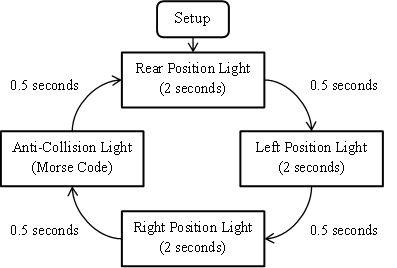
\includegraphics{Figures/LightsTestDiagram.png}
  \caption[Arduino\texttrademark Script Diagram]{Arduino\texttrademark Script Diagram}
  \label{fig:lightstestdiagram}
\end{figure}
The script 'DroneTest.ino' allows the subjects of the test to evaluate all lights on a straight line at several ranges between 50 and 350m, as shown in figure \ref{fig:ranges2}. To acquire the range during the test, an Android application was used, 'GPS Distance Location Tracker', which uses the GPS signal to track movement, including distances.\\
\begin{figure}[!htb]
  \centering
  \includegraphics[width=0.90\textwidth]{Figures/ranges2.png}
  \caption[Distances for Position and Anti-Collision lights range test]{Distances for Position and Anti-Collision lights range test}
  \label{fig:ranges2}
\end{figure}

In order to avoid fluctuations on the LEDs' intensity, a continuous power provider was used.\\
The test then consisted in each individual walking on a straight line, half towards and the other half away from the system to allow the subject to evaluate all LED separately, providing a qualitative evaluation (grade between 1 and 10). The test subjects gave an assessment of the lights intensity at the 50, 100, 150, 200, 250, 300 and 350m mark.\\

\section{Prototyping}
\label{section:pprototypes}

To provide an implementation example, the system will be adapted to a quadcopter.\\
Using the quadcopter's standard front side, the left and right position lights will be composed by 5 LEDs each to achieve a field coverage of 110\degree \citep{Easa2012}, where each LED overlaps the next one by 6\degree ; the rear position light will be composed by 8 LEDs to achieve a field coverage of 140\degree \citep{Easa2012}, where each LED overlaps the next one 3.4\degree . By overlapping LEDs, it is easier to ensure a complete field coverage, avoiding gaps caused by higher manufacture margins or defect's probability from the cheaper LEDs. Finally the anti-collision light will be composed by 3 LEDs, to concentrate the highest intensities of the LED around the aircraft and not on top of it. This configuration is shown in figure \ref{fig:esquemalights3}.\\

\begin{figure}[!htb]
  \centering
  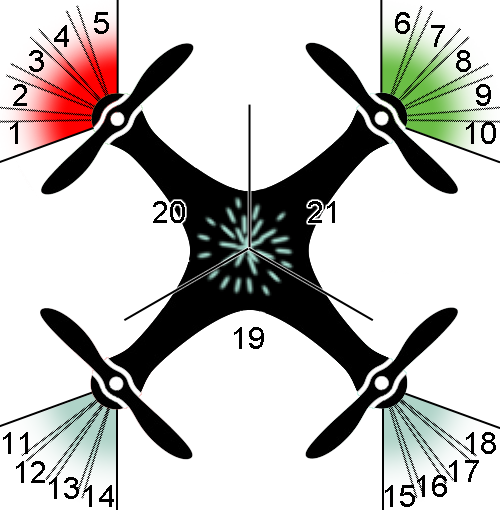
\includegraphics[width=0.6\textwidth]{Figures/esquemalights3.png}
  \caption[Configuration of Position and Anti-Collision on Quadcopter]{Configuration of Position and Anti-Collision on Quadcopter (1,2,3,4,5 - Left Position Light; 6,7,8,9,10 - Right Position Light; 11,12,13,14,15,16,17,18 - Rear Position Light; 19,20,21 - Anti-Collision Light}
  \label{fig:esquemalights3}
\end{figure}

To distribute power to all LEDs, a PCB was designed. As can be seen in figure \ref{fig:schematicluzes}, this board connects to the aircraft's power distribution board and to pin 13 of the Arduino\texttrademark Pro Mini.

\begin{figure}[!htb]
  \centering
  \includegraphics[width=0.80\textwidth]{Figures/schematicluzes.png}
  \caption[Schematic for Position and Anti-Collision Light System]{Schematic for Position and Anti-Collision Light System}
  \label{fig:schematicluzes}
\end{figure}

\subsection{Controlling the Anti-Collision LED}
\label{subsection:pcontrolblink}

To control the blinking pattern of the Anti-Collision LED, a simple C library was developed.\\
The script 'morseaircraft.h', contains all variables and functions available.\\
On 'morseaircraft.cpp', the function 'MorseAircraft', of the class with the same name, is given the type of aircraft, using the nomenclature explained in subsection \ref{subsection:aircraftypes} (for example 'H' for helicopters), when called. The function then provides the message that will be transmitted with the Anti-Collision Lights, the correct period for the Morse code, the number of bits transmitted (called order) and the type of aircraft coded in decimal base:
\begin{enumerate}
\setcounter{enumi}{-1}
\item A - Unpowered air sports
\item B - Hot air balloons
\item C - Cargo aircraft
\item[] ...
\setcounter{enumi}{11}
\item S - Powered air sports
\item T - Pressurized passenger aircraft required to carry ACAS
\item UA - Unmanned unpowered air sports
\item UB - Unmanned hot air balloons
\item[] ...
\setcounter{enumi}{26}
\item UT - Unmanned pressurized passenger aircraft required to carry ACAS
\end{enumerate}

The other function provided in 'morseaircraft.cpp' is flash() which controls the on and off times of the Anti-Collision Lights, correctly transmitting the Morse code. It will also rotate the message so that the least precedent bit always contains the bit that will be transmitted next.

\subsection{ISR's Quadcopter}
\label{subsection:pisr}

The visual spectrum solution was introduced on a quadcopter as implementation example, using the configuration shown in figure \ref{fig:esquemalights3} and the equipment from section \ref{section:pmaterial}.\\
The position lights were fixed to the bottom of the engines, to avoid interference with their operation. The anti-collision light was mounted on top of the IR sense and avoid prototype develop in chapter \ref{chapter:active}.\\
The equipped aircraft can be seen in figures~\ref{fig:visualprototype1}--\subref{fig:visualprototype2}, from its right side.\\
\begin{figure}[ht]
  \centering
  \subfigure[][]{
    \label{fig:visualprototype1} 
    \includegraphics[width=0.45\textwidth]{Figures/visualprototype1.png}
  }
  \hspace{8pt}
  \subfigure[][]{
    \label{fig:visualprototype2} 
    \includegraphics[width=0.45\textwidth]{Figures/visualprototype2.png} 
  }\\
  \caption[Aircraft with Visual Spectrum Solution Implemented]{Aircraft with visual spectrum solution implemented:
			\subref{fig:visualprototype1} with anti-collision light off; and,
			\subref{fig:visualprototype2} with anti-collision light on.}%
  \label{fig:visualprototype}%
\end{figure}

The total cost of the acquired material is \euro{20} with an included \euro{4} for miscellaneous material such as wire and solder.\\

After assembling the prototype on the quadcopter, the aircraft was flown in order to check the prototype behavior during flight, as shown in figures \ref{fig:visualground}--subref{fig:visualflight}.\\
\begin{figure}[ht]
  \centering
  \subfigure[][]{
    \label{fig:visualground} 
    \includegraphics[width=0.45\textwidth]{Figures/visualground.png}
  }
  \hspace{8pt}
  \subfigure[][]{
    \label{fig:visualflight} 
    \includegraphics[width=0.45\textwidth]{Figures/visualflying.png} 
  }\\
  \caption[Aircraft with Visual Spectrum Solution Implemented during Flight]{Aircraft with visual spectrum solution implemented during flight:
			\subref{fig:visualprototype1} ready for take-off; and,
			\subref{fig:visualprototype2} mid flight.}%
  \label{fig:visual}%
\end{figure}